\documentclass[1p]{elsarticle_modified}
%\bibliographystyle{elsarticle-num}

%\usepackage[colorlinks]{hyperref}
%\usepackage{abbrmath_seonhwa} %\Abb, \Ascr, \Acal ,\Abf, \Afrak
\usepackage{amsfonts}
\usepackage{amssymb}
\usepackage{amsmath}
\usepackage{amsthm}
\usepackage{scalefnt}
\usepackage{amsbsy}
\usepackage{kotex}
\usepackage{caption}
\usepackage{subfig}
\usepackage{color}
\usepackage{graphicx}
\usepackage{xcolor} %% white, black, red, green, blue, cyan, magenta, yellow
\usepackage{float}
\usepackage{setspace}
\usepackage{hyperref}

\usepackage{tikz}
\usetikzlibrary{arrows}

\usepackage{multirow}
\usepackage{array} % fixed length table
\usepackage{hhline}

%%%%%%%%%%%%%%%%%%%%%
\makeatletter
\renewcommand*\env@matrix[1][\arraystretch]{%
	\edef\arraystretch{#1}%
	\hskip -\arraycolsep
	\let\@ifnextchar\new@ifnextchar
	\array{*\c@MaxMatrixCols c}}
\makeatother %https://tex.stackexchange.com/questions/14071/how-can-i-increase-the-line-spacing-in-a-matrix
%%%%%%%%%%%%%%%

\usepackage[normalem]{ulem}

\newcommand{\msout}[1]{\ifmmode\text{\sout{\ensuremath{#1}}}\else\sout{#1}\fi}
%SOURCE: \msout is \stkout macro in https://tex.stackexchange.com/questions/20609/strikeout-in-math-mode

\newcommand{\cancel}[1]{
	\ifmmode
	{\color{red}\msout{#1}}
	\else
	{\color{red}\sout{#1}}
	\fi
}

\newcommand{\add}[1]{
	{\color{blue}\uwave{#1}}
}

\newcommand{\replace}[2]{
	\ifmmode
	{\color{red}\msout{#1}}{\color{blue}\uwave{#2}}
	\else
	{\color{red}\sout{#1}}{\color{blue}\uwave{#2}}
	\fi
}

\newcommand{\Sol}{\mathcal{S}} %segment
\newcommand{\D}{D} %diagram
\newcommand{\A}{\mathcal{A}} %arc


%%%%%%%%%%%%%%%%%%%%%%%%%%%%%5 test

\def\sl{\operatorname{\textup{SL}}(2,\Cbb)}
\def\psl{\operatorname{\textup{PSL}}(2,\Cbb)}
\def\quan{\mkern 1mu \triangleright \mkern 1mu}

\theoremstyle{definition}
\newtheorem{thm}{Theorem}[section]
\newtheorem{prop}[thm]{Proposition}
\newtheorem{lem}[thm]{Lemma}
\newtheorem{ques}[thm]{Question}
\newtheorem{cor}[thm]{Corollary}
\newtheorem{defn}[thm]{Definition}
\newtheorem{exam}[thm]{Example}
\newtheorem{rmk}[thm]{Remark}
\newtheorem{alg}[thm]{Algorithm}

\newcommand{\I}{\sqrt{-1}}
\begin{document}

%\begin{frontmatter}
%
%\title{Boundary parabolic representations of knots up to 8 crossings}
%
%%% Group authors per affiliation:
%\author{Yunhi Cho} 
%\address{Department of Mathematics, University of Seoul, Seoul, Korea}
%\ead{yhcho@uos.ac.kr}
%
%
%\author{Seonhwa Kim} %\fnref{s_kim}}
%\address{Center for Geometry and Physics, Institute for Basic Science, Pohang, 37673, Korea}
%\ead{ryeona17@ibs.re.kr}
%
%\author{Hyuk Kim}
%\address{Department of Mathematical Sciences, Seoul National University, Seoul 08826, Korea}
%\ead{hyukkim@snu.ac.kr}
%
%\author{Seokbeom Yoon}
%\address{Department of Mathematical Sciences, Seoul National University, Seoul, 08826,  Korea}
%\ead{sbyoon15@snu.ac.kr}
%
%\begin{abstract}
%We find all boundary parabolic representation of knots up to 8 crossings.
%
%\end{abstract}
%\begin{keyword}
%    \MSC[2010] 57M25 
%\end{keyword}
%
%\end{frontmatter}

%\linenumbers
%\tableofcontents
%
\newcommand\colored[1]{\textcolor{white}{\rule[-0.35ex]{0.8em}{1.4ex}}\kern-0.8em\color{red} #1}%
%\newcommand\colored[1]{\textcolor{white}{ #1}\kern-2.17ex	\textcolor{white}{ #1}\kern-1.81ex	\textcolor{white}{ #1}\kern-2.15ex\color{red}#1	}

{\Large $\underline{12n_{0132}~(K12n_{0132})}$}

\setlength{\tabcolsep}{10pt}
\renewcommand{\arraystretch}{1.6}
\vspace{1cm}\begin{tabular}{m{100pt}>{\centering\arraybackslash}m{274pt}}
\multirow{5}{120pt}{
	\centering
	\includegraphics[width=112pt]{../../../GIT/diagram.site/Diagrams/png/2221_12n_0132.png}\\
\ \ \ A knot diagram\footnotemark}&
\allowdisplaybreaks
\textbf{Linearized knot diagam} \\
\cline{2-2}
 &
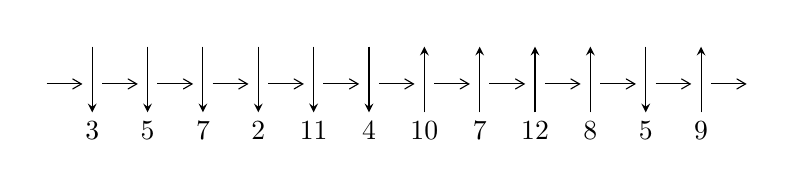
\begin{tikzpicture}[x=20pt, y=17pt]
	% nodes
	\node (C0) at (0, 0) {};
	\node (C1) at (1, 0) {};
	\node (C1U) at (1, +1) {};
	\node (C1D) at (1, -1) {3};

	\node (C2) at (2, 0) {};
	\node (C2U) at (2, +1) {};
	\node (C2D) at (2, -1) {5};

	\node (C3) at (3, 0) {};
	\node (C3U) at (3, +1) {};
	\node (C3D) at (3, -1) {7};

	\node (C4) at (4, 0) {};
	\node (C4U) at (4, +1) {};
	\node (C4D) at (4, -1) {2};

	\node (C5) at (5, 0) {};
	\node (C5U) at (5, +1) {};
	\node (C5D) at (5, -1) {11};

	\node (C6) at (6, 0) {};
	\node (C6U) at (6, +1) {};
	\node (C6D) at (6, -1) {4};

	\node (C7) at (7, 0) {};
	\node (C7U) at (7, +1) {};
	\node (C7D) at (7, -1) {10};

	\node (C8) at (8, 0) {};
	\node (C8U) at (8, +1) {};
	\node (C8D) at (8, -1) {7};

	\node (C9) at (9, 0) {};
	\node (C9U) at (9, +1) {};
	\node (C9D) at (9, -1) {12};

	\node (C10) at (10, 0) {};
	\node (C10U) at (10, +1) {};
	\node (C10D) at (10, -1) {8};

	\node (C11) at (11, 0) {};
	\node (C11U) at (11, +1) {};
	\node (C11D) at (11, -1) {5};

	\node (C12) at (12, 0) {};
	\node (C12U) at (12, +1) {};
	\node (C12D) at (12, -1) {9};
	\node (C13) at (13, 0) {};

	% arrows
	\draw[->,>={angle 60}]
	(C0) edge (C1) (C1) edge (C2) (C2) edge (C3) (C3) edge (C4) (C4) edge (C5) (C5) edge (C6) (C6) edge (C7) (C7) edge (C8) (C8) edge (C9) (C9) edge (C10) (C10) edge (C11) (C11) edge (C12) (C12) edge (C13) ;	\draw[->,>=stealth]
	(C1U) edge (C1D) (C2U) edge (C2D) (C3U) edge (C3D) (C4U) edge (C4D) (C5U) edge (C5D) (C6U) edge (C6D) (C7D) edge (C7U) (C8D) edge (C8U) (C9D) edge (C9U) (C10D) edge (C10U) (C11U) edge (C11D) (C12D) edge (C12U) ;
	\end{tikzpicture} \\
\hhline{~~} \\& 
\textbf{Solving Sequence} \\ \cline{2-2} 
 &
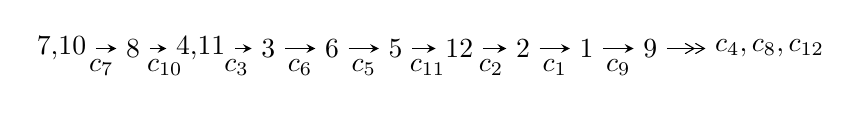
\begin{tikzpicture}[x=23pt, y=7pt]
	% node
	\node (A0) at (-1/8, 0) {7,10};
	\node (A1) at (1, 0) {8};
	\node (A2) at (33/16, 0) {4,11};
	\node (A3) at (25/8, 0) {3};
	\node (A4) at (33/8, 0) {6};
	\node (A5) at (41/8, 0) {5};
	\node (A6) at (49/8, 0) {12};
	\node (A7) at (57/8, 0) {2};
	\node (A8) at (65/8, 0) {1};
	\node (A9) at (73/8, 0) {9};
	\node (C1) at (1/2, -1) {$c_{7}$};
	\node (C2) at (3/2, -1) {$c_{10}$};
	\node (C3) at (21/8, -1) {$c_{3}$};
	\node (C4) at (29/8, -1) {$c_{6}$};
	\node (C5) at (37/8, -1) {$c_{5}$};
	\node (C6) at (45/8, -1) {$c_{11}$};
	\node (C7) at (53/8, -1) {$c_{2}$};
	\node (C8) at (61/8, -1) {$c_{1}$};
	\node (C9) at (69/8, -1) {$c_{9}$};
	\node (A10) at (11, 0) {$c_{4},c_{8},c_{12}$};

	% edge
	\draw[->,>=stealth]	
	(A0) edge (A1) (A1) edge (A2) (A2) edge (A3) (A3) edge (A4) (A4) edge (A5) (A5) edge (A6) (A6) edge (A7) (A7) edge (A8) (A8) edge (A9) ;
	\draw[->>,>={angle 60}]	
	(A9) edge (A10);
\end{tikzpicture} \\ 

\end{tabular} \\

\footnotetext{
The image of knot diagram is generated by the software ``\textbf{Draw programme}" developed by Andrew Bartholomew(\url{http://www.layer8.co.uk/maths/draw/index.htm\#Running-draw}), where we modified some parts for our purpose(\url{https://github.com/CATsTAILs/LinksPainter}).
}\phantom \\ \newline 
\centering \textbf{Ideals for irreducible components\footnotemark of $X_{\text{par}}$} 
 
\begin{align*}
I^u_{1}&=\langle 
-2.14796\times10^{52} u^{43}+9.58738\times10^{52} u^{42}+\cdots+1.56185\times10^{54} b+8.78201\times10^{53},\\
\phantom{I^u_{1}}&\phantom{= \langle  }-4.29892\times10^{54} u^{43}+3.28755\times10^{55} u^{42}+\cdots+1.56185\times10^{54} a+7.83354\times10^{55},\\
\phantom{I^u_{1}}&\phantom{= \langle  }u^{44}-7 u^{43}+\cdots-83 u-1\rangle \\
I^u_{2}&=\langle 
b,\;3 u^8-5 u^7- u^6+9 u^5-6 u^4-3 u^3+10 u^2+a-8 u+4,\;u^9- u^8-2 u^7+3 u^6+u^5-3 u^4+2 u^3- u+1\rangle \\
I^u_{3}&=\langle 
- u^2 a-2 u^2+b+1,\;a^2+a u+2 u^2+2 a-2 u+3,\;u^3- u^2+1\rangle \\
I^u_{4}&=\langle 
2 b+a-2,\;a^2-2 a-4,\;u+1\rangle \\
I^u_{5}&=\langle 
u^2+b,\;u^2+a-2 u+1,\;u^3- u^2+1\rangle \\
\\
\end{align*}
\raggedright * 5 irreducible components of $\dim_{\mathbb{C}}=0$, with total 64 representations.\\
\footnotetext{All coefficients of polynomials are rational numbers. But the coefficients are sometimes approximated in decimal forms when there is not enough margin.}
\newpage
\renewcommand{\arraystretch}{1}
\centering \section*{I. $I^u_{1}= \langle -2.15\times10^{52} u^{43}+9.59\times10^{52} u^{42}+\cdots+1.56\times10^{54} b+8.78\times10^{53},\;-4.30\times10^{54} u^{43}+3.29\times10^{55} u^{42}+\cdots+1.56\times10^{54} a+7.83\times10^{55},\;u^{44}-7 u^{43}+\cdots-83 u-1 \rangle$}
\flushleft \textbf{(i) Arc colorings}\\
\begin{tabular}{m{7pt} m{180pt} m{7pt} m{180pt} }
\flushright $a_{7}=$&$\begin{pmatrix}1\\0\end{pmatrix}$ \\
\flushright $a_{10}=$&$\begin{pmatrix}0\\u\end{pmatrix}$ \\
\flushright $a_{8}=$&$\begin{pmatrix}1\\- u^2\end{pmatrix}$ \\
\flushright $a_{4}=$&$\begin{pmatrix}2.75245 u^{43}-21.0490 u^{42}+\cdots-383.045 u-50.1555\\0.0137527 u^{43}-0.0613847 u^{42}+\cdots+4.13777 u-0.562282\end{pmatrix}$ \\
\flushright $a_{11}=$&$\begin{pmatrix}u\\- u^3+u\end{pmatrix}$ \\
\flushright $a_{3}=$&$\begin{pmatrix}2.76620 u^{43}-21.1104 u^{42}+\cdots-378.907 u-50.7178\\0.0137527 u^{43}-0.0613847 u^{42}+\cdots+4.13777 u-0.562282\end{pmatrix}$ \\
\flushright $a_{6}=$&$\begin{pmatrix}0.0964349 u^{43}-0.375473 u^{42}+\cdots-71.2040 u-27.7159\\-0.0727656 u^{43}+0.491309 u^{42}+\cdots-2.80714 u-0.409016\end{pmatrix}$ \\
\flushright $a_{5}=$&$\begin{pmatrix}0.102399 u^{43}-0.502049 u^{42}+\cdots-78.0105 u-27.7938\\-0.0451246 u^{43}+0.308080 u^{42}+\cdots-2.57914 u-0.402041\end{pmatrix}$ \\
\flushright $a_{12}=$&$\begin{pmatrix}-0.130388 u^{43}+0.959055 u^{42}+\cdots+40.6420 u+9.41950\\0.122234 u^{43}-0.687069 u^{42}+\cdots+11.8008 u+0.252623\end{pmatrix}$ \\
\flushright $a_{2}=$&$\begin{pmatrix}2.64549 u^{43}-20.3205 u^{42}+\cdots-328.997 u-32.6224\\-0.0451246 u^{43}+0.308080 u^{42}+\cdots-2.57914 u-0.402041\end{pmatrix}$ \\
\flushright $a_{1}=$&$\begin{pmatrix}0.124319 u^{43}-0.935985 u^{42}+\cdots-42.8904 u-9.55951\\-0.174640 u^{43}+1.02487 u^{42}+\cdots-12.6464 u-0.262253\end{pmatrix}$ \\
\flushright $a_{9}=$&$\begin{pmatrix}- u^2+1\\- u^2\end{pmatrix}$\\&\end{tabular}
\flushleft \textbf{(ii) Obstruction class $= -1$}\\~\\
\flushleft \textbf{(iii) Cusp Shapes $= -49.8054 u^{43}+389.878 u^{42}+\cdots+5096.96 u+52.1441$}\\~\\
\newpage\renewcommand{\arraystretch}{1}
\flushleft \textbf{(iv) u-Polynomials at the component}\newline \\
\begin{tabular}{m{50pt}|m{274pt}}
Crossings & \hspace{64pt}u-Polynomials at each crossing \\
\hline $$\begin{aligned}c_{1}\end{aligned}$$&$\begin{aligned}
&u^{44}+6 u^{43}+\cdots+29830 u+1
\end{aligned}$\\
\hline $$\begin{aligned}c_{2},c_{4}\end{aligned}$$&$\begin{aligned}
&u^{44}-14 u^{43}+\cdots-166 u-1
\end{aligned}$\\
\hline $$\begin{aligned}c_{3},c_{6}\end{aligned}$$&$\begin{aligned}
&u^{44}-5 u^{43}+\cdots+3072 u+512
\end{aligned}$\\
\hline $$\begin{aligned}c_{5},c_{11}\end{aligned}$$&$\begin{aligned}
&u^{44}-3 u^{43}+\cdots+4096 u-512
\end{aligned}$\\
\hline $$\begin{aligned}c_{7},c_{10}\end{aligned}$$&$\begin{aligned}
&u^{44}+7 u^{43}+\cdots+83 u-1
\end{aligned}$\\
\hline $$\begin{aligned}c_{8}\end{aligned}$$&$\begin{aligned}
&u^{44}-33 u^{43}+\cdots-6317 u+1
\end{aligned}$\\
\hline $$\begin{aligned}c_{9},c_{12}\end{aligned}$$&$\begin{aligned}
&u^{44}+5 u^{43}+\cdots-16 u-4
\end{aligned}$\\
\hline
\end{tabular}\\~\\
\newpage\renewcommand{\arraystretch}{1}
\flushleft \textbf{(v) Riley Polynomials at the component}\newline \\
\begin{tabular}{m{50pt}|m{274pt}}
Crossings & \hspace{64pt}Riley Polynomials at each crossing \\
\hline $$\begin{aligned}c_{1}\end{aligned}$$&$\begin{aligned}
&y^{44}+78 y^{43}+\cdots-889350874 y+1
\end{aligned}$\\
\hline $$\begin{aligned}c_{2},c_{4}\end{aligned}$$&$\begin{aligned}
&y^{44}-6 y^{43}+\cdots-29830 y+1
\end{aligned}$\\
\hline $$\begin{aligned}c_{3},c_{6}\end{aligned}$$&$\begin{aligned}
&y^{44}+63 y^{43}+\cdots-69206016 y+262144
\end{aligned}$\\
\hline $$\begin{aligned}c_{5},c_{11}\end{aligned}$$&$\begin{aligned}
&y^{44}+49 y^{43}+\cdots-15859712 y+262144
\end{aligned}$\\
\hline $$\begin{aligned}c_{7},c_{10}\end{aligned}$$&$\begin{aligned}
&y^{44}-33 y^{43}+\cdots-6317 y+1
\end{aligned}$\\
\hline $$\begin{aligned}c_{8}\end{aligned}$$&$\begin{aligned}
&y^{44}-37 y^{43}+\cdots-39734481 y+1
\end{aligned}$\\
\hline $$\begin{aligned}c_{9},c_{12}\end{aligned}$$&$\begin{aligned}
&y^{44}-3 y^{43}+\cdots-1304 y+16
\end{aligned}$\\
\hline
\end{tabular}\\~\\
\newpage\flushleft \textbf{(vi) Complex Volumes and Cusp Shapes}
$$\begin{array}{c|c|c}  
\text{Solutions to }I^u_{1}& \I (\text{vol} + \sqrt{-1}CS) & \text{Cusp shape}\\
 \hline 
\begin{aligned}
u &= -0.876497 + 0.429976 I \\
a &= -0.802254 - 0.743828 I \\
b &= \phantom{-}0.076755 - 1.159430 I\end{aligned}
 & \phantom{-}3.87014 - 2.97279 I & \phantom{-}3.60919 + 6.63471 I \\ \hline\begin{aligned}
u &= -0.876497 - 0.429976 I \\
a &= -0.802254 + 0.743828 I \\
b &= \phantom{-}0.076755 + 1.159430 I\end{aligned}
 & \phantom{-}3.87014 + 2.97279 I & \phantom{-}3.60919 - 6.63471 I \\ \hline\begin{aligned}
u &= -1.035690 + 0.011118 I \\
a &= \phantom{-}0.98809 - 3.01949 I \\
b &= -0.626019 - 0.060302 I\end{aligned}
 & \phantom{-}0.651471 + 0.106624 I & -43.8474 - 14.3936 I \\ \hline\begin{aligned}
u &= -1.035690 - 0.011118 I \\
a &= \phantom{-}0.98809 + 3.01949 I \\
b &= -0.626019 + 0.060302 I\end{aligned}
 & \phantom{-}0.651471 - 0.106624 I & -43.8474 + 14.3936 I \\ \hline\begin{aligned}
u &= \phantom{-}1.04545\phantom{ +0.000000I} \\
a &= -1.23357\phantom{ +0.000000I} \\
b &= \phantom{-}1.68917\phantom{ +0.000000I}\end{aligned}
 & -7.14674\phantom{ +0.000000I} & \phantom{-}39.2060\phantom{ +0.000000I} \\ \hline\begin{aligned}
u &= \phantom{-}0.638907 + 0.623619 I \\
a &= \phantom{-}0.054165 - 0.369885 I \\
b &= -0.199038 + 0.637626 I\end{aligned}
 & -2.03545 + 1.53423 I & -2.10831 - 3.28440 I \\ \hline\begin{aligned}
u &= \phantom{-}0.638907 - 0.623619 I \\
a &= \phantom{-}0.054165 + 0.369885 I \\
b &= -0.199038 - 0.637626 I\end{aligned}
 & -2.03545 - 1.53423 I & -2.10831 + 3.28440 I \\ \hline\begin{aligned}
u &= -0.354769 + 0.792242 I \\
a &= \phantom{-}1.153100 + 0.457040 I \\
b &= \phantom{-}0.884926 + 0.773845 I\end{aligned}
 & \phantom{-}2.35471 - 1.62269 I & \phantom{-}0.78025 + 2.86308 I \\ \hline\begin{aligned}
u &= -0.354769 - 0.792242 I \\
a &= \phantom{-}1.153100 - 0.457040 I \\
b &= \phantom{-}0.884926 - 0.773845 I\end{aligned}
 & \phantom{-}2.35471 + 1.62269 I & \phantom{-}0.78025 - 2.86308 I \\ \hline\begin{aligned}
u &= \phantom{-}0.883739 + 0.725281 I \\
a &= \phantom{-}2.46589 + 0.69772 I \\
b &= \phantom{-}0.500417 - 0.051284 I\end{aligned}
 & -4.23715 + 2.76938 I & -48.8073 + 0. I\phantom{ +0.000000I}\\
 \hline 
 \end{array}$$\newpage$$\begin{array}{c|c|c}  
\text{Solutions to }I^u_{1}& \I (\text{vol} + \sqrt{-1}CS) & \text{Cusp shape}\\
 \hline 
\begin{aligned}
u &= \phantom{-}0.883739 - 0.725281 I \\
a &= \phantom{-}2.46589 - 0.69772 I \\
b &= \phantom{-}0.500417 + 0.051284 I\end{aligned}
 & -4.23715 - 2.76938 I & -48.8073 + 0. I\phantom{ +0.000000I} \\ \hline\begin{aligned}
u &= -0.833904\phantom{ +0.000000I} \\
a &= \phantom{-}0.838853\phantom{ +0.000000I} \\
b &= -0.0760954\phantom{ +0.000000I}\end{aligned}
 & \phantom{-}1.20368\phantom{ +0.000000I} & \phantom{-}8.97050\phantom{ +0.000000I} \\ \hline\begin{aligned}
u &= -0.806388\phantom{ +0.000000I} \\
a &= \phantom{-}17.4240\phantom{ +0.000000I} \\
b &= \phantom{-}0.105321\phantom{ +0.000000I}\end{aligned}
 & -0.460937\phantom{ +0.000000I} & -368.890\phantom{ +0.000000I} \\ \hline\begin{aligned}
u &= \phantom{-}1.112660 + 0.494049 I \\
a &= -0.401224 - 0.346268 I \\
b &= -0.297482 + 0.701848 I\end{aligned}
 & \phantom{-}2.13500 + 7.76603 I & \phantom{-0.000000 } 0 \\ \hline\begin{aligned}
u &= \phantom{-}1.112660 - 0.494049 I \\
a &= -0.401224 + 0.346268 I \\
b &= -0.297482 - 0.701848 I\end{aligned}
 & \phantom{-}2.13500 - 7.76603 I & \phantom{-0.000000 } 0 \\ \hline\begin{aligned}
u &= \phantom{-}0.309756 + 0.710019 I \\
a &= \phantom{-}0.447198 - 0.401576 I \\
b &= -0.053147 - 0.769930 I\end{aligned}
 & -0.22354 - 3.19884 I & \phantom{-}0.00447 + 5.55216 I \\ \hline\begin{aligned}
u &= \phantom{-}0.309756 - 0.710019 I \\
a &= \phantom{-}0.447198 + 0.401576 I \\
b &= -0.053147 + 0.769930 I\end{aligned}
 & -0.22354 + 3.19884 I & \phantom{-}0.00447 - 5.55216 I \\ \hline\begin{aligned}
u &= \phantom{-}0.073729 + 1.240780 I \\
a &= \phantom{-}0.379736 + 0.020924 I \\
b &= \phantom{-}0.63482 + 1.93161 I\end{aligned}
 & \phantom{-}10.77560 - 8.87064 I & \phantom{-0.000000 } 0 \\ \hline\begin{aligned}
u &= \phantom{-}0.073729 - 1.240780 I \\
a &= \phantom{-}0.379736 - 0.020924 I \\
b &= \phantom{-}0.63482 - 1.93161 I\end{aligned}
 & \phantom{-}10.77560 + 8.87064 I & \phantom{-0.000000 } 0 \\ \hline\begin{aligned}
u &= -0.132383 + 1.258200 I \\
a &= \phantom{-}0.0707679 - 0.1181420 I \\
b &= \phantom{-}0.10550 - 2.15662 I\end{aligned}
 & \phantom{-}11.64120 - 0.54721 I & \phantom{-0.000000 } 0\\
 \hline 
 \end{array}$$\newpage$$\begin{array}{c|c|c}  
\text{Solutions to }I^u_{1}& \I (\text{vol} + \sqrt{-1}CS) & \text{Cusp shape}\\
 \hline 
\begin{aligned}
u &= -0.132383 - 1.258200 I \\
a &= \phantom{-}0.0707679 + 0.1181420 I \\
b &= \phantom{-}0.10550 + 2.15662 I\end{aligned}
 & \phantom{-}11.64120 + 0.54721 I & \phantom{-0.000000 } 0 \\ \hline\begin{aligned}
u &= \phantom{-}1.118360 + 0.595860 I \\
a &= \phantom{-}0.909006 + 0.370619 I \\
b &= -0.644410 - 1.075560 I\end{aligned}
 & -0.60424 + 3.28908 I & \phantom{-0.000000 } 0 \\ \hline\begin{aligned}
u &= \phantom{-}1.118360 - 0.595860 I \\
a &= \phantom{-}0.909006 - 0.370619 I \\
b &= -0.644410 + 1.075560 I\end{aligned}
 & -0.60424 - 3.28908 I & \phantom{-0.000000 } 0 \\ \hline\begin{aligned}
u &= -1.353770 + 0.147916 I \\
a &= \phantom{-}0.380791 - 1.326250 I \\
b &= \phantom{-}0.573832 + 1.158340 I\end{aligned}
 & \phantom{-}5.03100 + 0.55063 I & \phantom{-0.000000 } 0 \\ \hline\begin{aligned}
u &= -1.353770 - 0.147916 I \\
a &= \phantom{-}0.380791 + 1.326250 I \\
b &= \phantom{-}0.573832 - 1.158340 I\end{aligned}
 & \phantom{-}5.03100 - 0.55063 I & \phantom{-0.000000 } 0 \\ \hline\begin{aligned}
u &= -0.608345 + 0.151373 I \\
a &= -0.48220 - 1.88435 I \\
b &= -0.158567 - 1.356840 I\end{aligned}
 & \phantom{-}4.00876 - 2.95005 I & -9.2752 + 14.0588 I \\ \hline\begin{aligned}
u &= -0.608345 - 0.151373 I \\
a &= -0.48220 + 1.88435 I \\
b &= -0.158567 + 1.356840 I\end{aligned}
 & \phantom{-}4.00876 + 2.95005 I & -9.2752 - 14.0588 I \\ \hline\begin{aligned}
u &= \phantom{-}1.405350 + 0.093871 I \\
a &= \phantom{-}0.454924 + 1.244670 I \\
b &= -1.19138 - 1.51744 I\end{aligned}
 & \phantom{-}4.40564 + 2.10618 I & \phantom{-0.000000 } 0 \\ \hline\begin{aligned}
u &= \phantom{-}1.405350 - 0.093871 I \\
a &= \phantom{-}0.454924 - 1.244670 I \\
b &= -1.19138 + 1.51744 I\end{aligned}
 & \phantom{-}4.40564 - 2.10618 I & \phantom{-0.000000 } 0 \\ \hline\begin{aligned}
u &= \phantom{-}1.45332 + 0.14450 I \\
a &= -0.11796 - 1.93576 I \\
b &= -0.46438 + 2.32992 I\end{aligned}
 & \phantom{-}10.46410 + 4.58464 I & \phantom{-0.000000 } 0\\
 \hline 
 \end{array}$$\newpage$$\begin{array}{c|c|c}  
\text{Solutions to }I^u_{1}& \I (\text{vol} + \sqrt{-1}CS) & \text{Cusp shape}\\
 \hline 
\begin{aligned}
u &= \phantom{-}1.45332 - 0.14450 I \\
a &= -0.11796 + 1.93576 I \\
b &= -0.46438 - 2.32992 I\end{aligned}
 & \phantom{-}10.46410 - 4.58464 I & \phantom{-0.000000 } 0 \\ \hline\begin{aligned}
u &= \phantom{-}1.46913 + 0.29367 I \\
a &= -0.488382 + 0.902569 I \\
b &= \phantom{-}1.91388 - 0.67361 I\end{aligned}
 & \phantom{-}8.25016 + 5.56575 I & \phantom{-0.000000 } 0 \\ \hline\begin{aligned}
u &= \phantom{-}1.46913 - 0.29367 I \\
a &= -0.488382 - 0.902569 I \\
b &= \phantom{-}1.91388 + 0.67361 I\end{aligned}
 & \phantom{-}8.25016 - 5.56575 I & \phantom{-0.000000 } 0 \\ \hline\begin{aligned}
u &= \phantom{-}1.40535 + 0.62626 I \\
a &= \phantom{-}1.00047 + 1.55409 I \\
b &= \phantom{-}0.88791 - 1.82835 I\end{aligned}
 & \phantom{-}14.9516 + 15.4441 I & \phantom{-0.000000 } 0 \\ \hline\begin{aligned}
u &= \phantom{-}1.40535 - 0.62626 I \\
a &= \phantom{-}1.00047 - 1.55409 I \\
b &= \phantom{-}0.88791 + 1.82835 I\end{aligned}
 & \phantom{-}14.9516 - 15.4441 I & \phantom{-0.000000 } 0 \\ \hline\begin{aligned}
u &= -1.41723 + 0.69052 I \\
a &= \phantom{-}1.12597 - 1.25429 I \\
b &= \phantom{-}0.53080 + 2.12848 I\end{aligned}
 & \phantom{-}15.5975 - 6.3488 I & \phantom{-0.000000 } 0 \\ \hline\begin{aligned}
u &= -1.41723 - 0.69052 I \\
a &= \phantom{-}1.12597 + 1.25429 I \\
b &= \phantom{-}0.53080 - 2.12848 I\end{aligned}
 & \phantom{-}15.5975 + 6.3488 I & \phantom{-0.000000 } 0 \\ \hline\begin{aligned}
u &= \phantom{-}1.51754 + 0.53920 I \\
a &= -0.84332 - 1.48882 I \\
b &= -0.35692 + 2.33329 I\end{aligned}
 & \phantom{-}16.9016 + 6.9619 I & \phantom{-0.000000 } 0 \\ \hline\begin{aligned}
u &= \phantom{-}1.51754 - 0.53920 I \\
a &= -0.84332 + 1.48882 I \\
b &= -0.35692 - 2.33329 I\end{aligned}
 & \phantom{-}16.9016 - 6.9619 I & \phantom{-0.000000 } 0 \\ \hline\begin{aligned}
u &= -0.270791 + 0.261743 I \\
a &= -4.22835 + 0.15470 I \\
b &= -0.526256 + 0.439239 I\end{aligned}
 & -0.967972 - 0.798268 I & -5.17338 - 0.48170 I\\
 \hline 
 \end{array}$$\newpage$$\begin{array}{c|c|c}  
\text{Solutions to }I^u_{1}& \I (\text{vol} + \sqrt{-1}CS) & \text{Cusp shape}\\
 \hline 
\begin{aligned}
u &= -0.270791 - 0.261743 I \\
a &= -4.22835 - 0.15470 I \\
b &= -0.526256 - 0.439239 I\end{aligned}
 & -0.967972 + 0.798268 I & -5.17338 + 0.48170 I \\ \hline\begin{aligned}
u &= -1.53465 + 0.55119 I \\
a &= -0.87468 + 1.14741 I \\
b &= \phantom{-}0.35572 - 2.21568 I\end{aligned}
 & \phantom{-}15.8788 + 2.3692 I & \phantom{-0.000000 } 0 \\ \hline\begin{aligned}
u &= -1.53465 - 0.55119 I \\
a &= -0.87468 - 1.14741 I \\
b &= \phantom{-}0.35572 + 2.21568 I\end{aligned}
 & \phantom{-}15.8788 - 2.3692 I & \phantom{-0.000000 } 0 \\ \hline\begin{aligned}
u &= -0.0125953\phantom{ +0.000000I} \\
a &= -45.4128\phantom{ +0.000000I} \\
b &= -0.612334\phantom{ +0.000000I}\end{aligned}
 & -1.00318\phantom{ +0.000000I} & -10.1720\phantom{ +0.000000I}\\
 \hline 
 \end{array}$$\newpage\newpage\renewcommand{\arraystretch}{1}
\centering \section*{II. $I^u_{2}= \langle b,\;3 u^8-5 u^7+\cdots+a+4,\;u^9- u^8-2 u^7+3 u^6+u^5-3 u^4+2 u^3- u+1 \rangle$}
\flushleft \textbf{(i) Arc colorings}\\
\begin{tabular}{m{7pt} m{180pt} m{7pt} m{180pt} }
\flushright $a_{7}=$&$\begin{pmatrix}1\\0\end{pmatrix}$ \\
\flushright $a_{10}=$&$\begin{pmatrix}0\\u\end{pmatrix}$ \\
\flushright $a_{8}=$&$\begin{pmatrix}1\\- u^2\end{pmatrix}$ \\
\flushright $a_{4}=$&$\begin{pmatrix}-3 u^8+5 u^7+u^6-9 u^5+6 u^4+3 u^3-10 u^2+8 u-4\\0\end{pmatrix}$ \\
\flushright $a_{11}=$&$\begin{pmatrix}u\\- u^3+u\end{pmatrix}$ \\
\flushright $a_{3}=$&$\begin{pmatrix}-3 u^8+5 u^7+u^6-9 u^5+6 u^4+3 u^3-10 u^2+8 u-4\\0\end{pmatrix}$ \\
\flushright $a_{6}=$&$\begin{pmatrix}1\\0\end{pmatrix}$ \\
\flushright $a_{5}=$&$\begin{pmatrix}u^4- u^2+1\\- u^6+2 u^4- u^2\end{pmatrix}$ \\
\flushright $a_{12}=$&$\begin{pmatrix}u^7-2 u^5+2 u^3\\- u^8+u^7+3 u^6-2 u^5-3 u^4+2 u^3+1\end{pmatrix}$ \\
\flushright $a_{2}=$&$\begin{pmatrix}-3 u^8+5 u^7+u^6-9 u^5+5 u^4+3 u^3-9 u^2+8 u-5\\u^6-2 u^4+u^2\end{pmatrix}$ \\
\flushright $a_{1}=$&$\begin{pmatrix}- u^4+u^2-1\\u^6-2 u^4+u^2\end{pmatrix}$ \\
\flushright $a_{9}=$&$\begin{pmatrix}- u^2+1\\- u^2\end{pmatrix}$\\&\end{tabular}
\flushleft \textbf{(ii) Obstruction class $= 1$}\\~\\
\flushleft \textbf{(iii) Cusp Shapes $= 42 u^8-82 u^7-19 u^6+153 u^5-83 u^4-70 u^3+143 u^2-120 u+48$}\\~\\
\newpage\renewcommand{\arraystretch}{1}
\flushleft \textbf{(iv) u-Polynomials at the component}\newline \\
\begin{tabular}{m{50pt}|m{274pt}}
Crossings & \hspace{64pt}u-Polynomials at each crossing \\
\hline $$\begin{aligned}c_{1},c_{2}\end{aligned}$$&$\begin{aligned}
&(u-1)^9
\end{aligned}$\\
\hline $$\begin{aligned}c_{3},c_{6}\end{aligned}$$&$\begin{aligned}
&u^9
\end{aligned}$\\
\hline $$\begin{aligned}c_{4}\end{aligned}$$&$\begin{aligned}
&(u+1)^9
\end{aligned}$\\
\hline $$\begin{aligned}c_{5}\end{aligned}$$&$\begin{aligned}
&u^9-3 u^8+8 u^7-13 u^6+17 u^5-17 u^4+12 u^3-6 u^2+u+1
\end{aligned}$\\
\hline $$\begin{aligned}c_{7}\end{aligned}$$&$\begin{aligned}
&u^9- u^8-2 u^7+3 u^6+u^5-3 u^4+2 u^3- u+1
\end{aligned}$\\
\hline $$\begin{aligned}c_{8}\end{aligned}$$&$\begin{aligned}
&u^9-5 u^8+12 u^7-15 u^6+9 u^5+u^4-4 u^3+2 u^2+u-1
\end{aligned}$\\
\hline $$\begin{aligned}c_{9}\end{aligned}$$&$\begin{aligned}
&u^9- u^8+2 u^7- u^6+3 u^5- u^4+2 u^3+u+1
\end{aligned}$\\
\hline $$\begin{aligned}c_{10}\end{aligned}$$&$\begin{aligned}
&u^9+u^8-2 u^7-3 u^6+u^5+3 u^4+2 u^3- u-1
\end{aligned}$\\
\hline $$\begin{aligned}c_{11}\end{aligned}$$&$\begin{aligned}
&u^9+3 u^8+8 u^7+13 u^6+17 u^5+17 u^4+12 u^3+6 u^2+u-1
\end{aligned}$\\
\hline $$\begin{aligned}c_{12}\end{aligned}$$&$\begin{aligned}
&u^9+u^8+2 u^7+u^6+3 u^5+u^4+2 u^3+u-1
\end{aligned}$\\
\hline
\end{tabular}\\~\\
\newpage\renewcommand{\arraystretch}{1}
\flushleft \textbf{(v) Riley Polynomials at the component}\newline \\
\begin{tabular}{m{50pt}|m{274pt}}
Crossings & \hspace{64pt}Riley Polynomials at each crossing \\
\hline $$\begin{aligned}c_{1},c_{2},c_{4}\end{aligned}$$&$\begin{aligned}
&(y-1)^9
\end{aligned}$\\
\hline $$\begin{aligned}c_{3},c_{6}\end{aligned}$$&$\begin{aligned}
&y^9
\end{aligned}$\\
\hline $$\begin{aligned}c_{5},c_{11}\end{aligned}$$&$\begin{aligned}
&y^9+7 y^8+20 y^7+25 y^6+5 y^5-15 y^4+22 y^2+13 y-1
\end{aligned}$\\
\hline $$\begin{aligned}c_{7},c_{10}\end{aligned}$$&$\begin{aligned}
&y^9-5 y^8+12 y^7-15 y^6+9 y^5+y^4-4 y^3+2 y^2+y-1
\end{aligned}$\\
\hline $$\begin{aligned}c_{8}\end{aligned}$$&$\begin{aligned}
&y^9- y^8+12 y^7-7 y^6+37 y^5+y^4-10 y^2+5 y-1
\end{aligned}$\\
\hline $$\begin{aligned}c_{9},c_{12}\end{aligned}$$&$\begin{aligned}
&y^9+3 y^8+8 y^7+13 y^6+17 y^5+17 y^4+12 y^3+6 y^2+y-1
\end{aligned}$\\
\hline
\end{tabular}\\~\\
\newpage\flushleft \textbf{(vi) Complex Volumes and Cusp Shapes}
$$\begin{array}{c|c|c}  
\text{Solutions to }I^u_{2}& \I (\text{vol} + \sqrt{-1}CS) & \text{Cusp shape}\\
 \hline 
\begin{aligned}
u &= \phantom{-}0.772920 + 0.510351 I \\
a &= -0.920144 - 0.598375 I \\
b &= \phantom{-0.000000 } 0\end{aligned}
 & -3.42837 + 2.09337 I & -7.68972 - 3.82038 I \\ \hline\begin{aligned}
u &= \phantom{-}0.772920 - 0.510351 I \\
a &= -0.920144 + 0.598375 I \\
b &= \phantom{-0.000000 } 0\end{aligned}
 & -3.42837 - 2.09337 I & -7.68972 + 3.82038 I \\ \hline\begin{aligned}
u &= -0.825933\phantom{ +0.000000I} \\
a &= -14.5113\phantom{ +0.000000I} \\
b &= \phantom{-0.000000 } 0\end{aligned}
 & -0.446489\phantom{ +0.000000I} & \phantom{-}211.240\phantom{ +0.000000I} \\ \hline\begin{aligned}
u &= -1.173910 + 0.391555 I \\
a &= \phantom{-}0.719281 + 0.119276 I \\
b &= \phantom{-0.000000 } 0\end{aligned}
 & \phantom{-}2.72642 - 1.33617 I & \phantom{-}1.56769 + 0.26615 I \\ \hline\begin{aligned}
u &= -1.173910 - 0.391555 I \\
a &= \phantom{-}0.719281 - 0.119276 I \\
b &= \phantom{-0.000000 } 0\end{aligned}
 & \phantom{-}2.72642 + 1.33617 I & \phantom{-}1.56769 - 0.26615 I \\ \hline\begin{aligned}
u &= \phantom{-}0.141484 + 0.739668 I \\
a &= \phantom{-}0.590648 + 0.449402 I \\
b &= \phantom{-0.000000 } 0\end{aligned}
 & -1.02799 - 2.45442 I & -5.04100 + 1.69416 I \\ \hline\begin{aligned}
u &= \phantom{-}0.141484 - 0.739668 I \\
a &= \phantom{-}0.590648 - 0.449402 I \\
b &= \phantom{-0.000000 } 0\end{aligned}
 & -1.02799 + 2.45442 I & -5.04100 - 1.69416 I \\ \hline\begin{aligned}
u &= \phantom{-}1.172470 + 0.500383 I \\
a &= \phantom{-}0.365868 - 0.247975 I \\
b &= \phantom{-0.000000 } 0\end{aligned}
 & \phantom{-}1.95319 + 7.08493 I & -0.45449 - 1.34000 I \\ \hline\begin{aligned}
u &= \phantom{-}1.172470 - 0.500383 I \\
a &= \phantom{-}0.365868 + 0.247975 I \\
b &= \phantom{-0.000000 } 0\end{aligned}
 & \phantom{-}1.95319 - 7.08493 I & -0.45449 + 1.34000 I\\
 \hline 
 \end{array}$$\newpage\newpage\renewcommand{\arraystretch}{1}
\centering \section*{III. $I^u_{3}= \langle - u^2 a-2 u^2+b+1,\;a^2+a u+2 u^2+2 a-2 u+3,\;u^3- u^2+1 \rangle$}
\flushleft \textbf{(i) Arc colorings}\\
\begin{tabular}{m{7pt} m{180pt} m{7pt} m{180pt} }
\flushright $a_{7}=$&$\begin{pmatrix}1\\0\end{pmatrix}$ \\
\flushright $a_{10}=$&$\begin{pmatrix}0\\u\end{pmatrix}$ \\
\flushright $a_{8}=$&$\begin{pmatrix}1\\- u^2\end{pmatrix}$ \\
\flushright $a_{4}=$&$\begin{pmatrix}a\\u^2 a+2 u^2-1\end{pmatrix}$ \\
\flushright $a_{11}=$&$\begin{pmatrix}u\\- u^2+u+1\end{pmatrix}$ \\
\flushright $a_{3}=$&$\begin{pmatrix}u^2 a+2 u^2+a-1\\u^2 a+2 u^2-1\end{pmatrix}$ \\
\flushright $a_{6}=$&$\begin{pmatrix}u^2 a+3 u^2-2 u+1\\a u+u^2+a+u+2\end{pmatrix}$ \\
\flushright $a_{5}=$&$\begin{pmatrix}u^2 a+3 u^2-2 u+1\\a u+u^2+a+u+2\end{pmatrix}$ \\
\flushright $a_{12}=$&$\begin{pmatrix}u\\- u^2+u+1\end{pmatrix}$ \\
\flushright $a_{2}=$&$\begin{pmatrix}u^2 a+a u+4 u^2+a- u+1\\a u+u^2+a+u+2\end{pmatrix}$ \\
\flushright $a_{1}=$&$\begin{pmatrix}-1\\0\end{pmatrix}$ \\
\flushright $a_{9}=$&$\begin{pmatrix}- u^2+1\\- u^2\end{pmatrix}$\\&\end{tabular}
\flushleft \textbf{(ii) Obstruction class $= 1$}\\~\\
\flushleft \textbf{(iii) Cusp Shapes $= 16 u^2 a-11 a u+16 u^2-11 a-30 u$}\\~\\
\newpage\renewcommand{\arraystretch}{1}
\flushleft \textbf{(iv) u-Polynomials at the component}\newline \\
\begin{tabular}{m{50pt}|m{274pt}}
Crossings & \hspace{64pt}u-Polynomials at each crossing \\
\hline $$\begin{aligned}c_{1},c_{3},c_{8}\\c_{12}\end{aligned}$$&$\begin{aligned}
&(u^3- u^2+2 u-1)^2
\end{aligned}$\\
\hline $$\begin{aligned}c_{2},c_{10}\end{aligned}$$&$\begin{aligned}
&(u^3+u^2-1)^2
\end{aligned}$\\
\hline $$\begin{aligned}c_{4},c_{7}\end{aligned}$$&$\begin{aligned}
&(u^3- u^2+1)^2
\end{aligned}$\\
\hline $$\begin{aligned}c_{5},c_{11}\end{aligned}$$&$\begin{aligned}
&u^6
\end{aligned}$\\
\hline $$\begin{aligned}c_{6},c_{9}\end{aligned}$$&$\begin{aligned}
&(u^3+u^2+2 u+1)^2
\end{aligned}$\\
\hline
\end{tabular}\\~\\
\newpage\renewcommand{\arraystretch}{1}
\flushleft \textbf{(v) Riley Polynomials at the component}\newline \\
\begin{tabular}{m{50pt}|m{274pt}}
Crossings & \hspace{64pt}Riley Polynomials at each crossing \\
\hline $$\begin{aligned}c_{1},c_{3},c_{6}\\c_{8},c_{9},c_{12}\end{aligned}$$&$\begin{aligned}
&(y^3+3 y^2+2 y-1)^2
\end{aligned}$\\
\hline $$\begin{aligned}c_{2},c_{4},c_{7}\\c_{10}\end{aligned}$$&$\begin{aligned}
&(y^3- y^2+2 y-1)^2
\end{aligned}$\\
\hline $$\begin{aligned}c_{5},c_{11}\end{aligned}$$&$\begin{aligned}
&y^6
\end{aligned}$\\
\hline
\end{tabular}\\~\\
\newpage\flushleft \textbf{(vi) Complex Volumes and Cusp Shapes}
$$\begin{array}{c|c|c}  
\text{Solutions to }I^u_{3}& \I (\text{vol} + \sqrt{-1}CS) & \text{Cusp shape}\\
 \hline 
\begin{aligned}
u &= \phantom{-}0.877439 + 0.744862 I \\
a &= -0.930160 - 0.424452 I \\
b &= -0.215080 + 1.307140 I\end{aligned}
 & \phantom{-0.000000 -}5.65624 I & -1.47396 - 5.95889 I \\ \hline\begin{aligned}
u &= \phantom{-}0.877439 + 0.744862 I \\
a &= -1.94728 - 0.32041 I \\
b &= -0.569840\phantom{ +0.000000I}\end{aligned}
 & -4.13758 + 2.82812 I & \phantom{-}14.7077 - 20.6881 I \\ \hline\begin{aligned}
u &= \phantom{-}0.877439 - 0.744862 I \\
a &= -0.930160 + 0.424452 I \\
b &= -0.215080 - 1.307140 I\end{aligned}
 & \phantom{-0.000000 } -5.65624 I & -1.47396 + 5.95889 I \\ \hline\begin{aligned}
u &= \phantom{-}0.877439 - 0.744862 I \\
a &= -1.94728 + 0.32041 I \\
b &= -0.569840\phantom{ +0.000000I}\end{aligned}
 & -4.13758 - 2.82812 I & \phantom{-}14.7077 + 20.6881 I \\ \hline\begin{aligned}
u &= -0.754878\phantom{ +0.000000I} \\
a &= -0.62256 + 2.29387 I \\
b &= -0.215080 + 1.307140 I\end{aligned}
 & \phantom{-}4.13758 + 2.82812 I & \phantom{-}27.7662 + 14.7292 I \\ \hline\begin{aligned}
u &= -0.754878\phantom{ +0.000000I} \\
a &= -0.62256 - 2.29387 I \\
b &= -0.215080 - 1.307140 I\end{aligned}
 & \phantom{-}4.13758 - 2.82812 I & \phantom{-}27.7662 - 14.7292 I\\
 \hline 
 \end{array}$$\newpage\newpage\renewcommand{\arraystretch}{1}
\centering \section*{IV. $I^u_{4}= \langle 2 b+a-2,\;a^2-2 a-4,\;u+1 \rangle$}
\flushleft \textbf{(i) Arc colorings}\\
\begin{tabular}{m{7pt} m{180pt} m{7pt} m{180pt} }
\flushright $a_{7}=$&$\begin{pmatrix}1\\0\end{pmatrix}$ \\
\flushright $a_{10}=$&$\begin{pmatrix}0\\-1\end{pmatrix}$ \\
\flushright $a_{8}=$&$\begin{pmatrix}1\\-1\end{pmatrix}$ \\
\flushright $a_{4}=$&$\begin{pmatrix}a\\-\frac{1}{2} a+1\end{pmatrix}$ \\
\flushright $a_{11}=$&$\begin{pmatrix}-1\\0\end{pmatrix}$ \\
\flushright $a_{3}=$&$\begin{pmatrix}\frac{1}{2} a+1\\-\frac{1}{2} a+1\end{pmatrix}$ \\
\flushright $a_{6}=$&$\begin{pmatrix}3\\\frac{1}{2} a-2\end{pmatrix}$ \\
\flushright $a_{5}=$&$\begin{pmatrix}\frac{1}{2} a+1\\\frac{1}{2} a-2\end{pmatrix}$ \\
\flushright $a_{12}=$&$\begin{pmatrix}0\\\frac{3}{2} a-5\end{pmatrix}$ \\
\flushright $a_{2}=$&$\begin{pmatrix}1\\\frac{1}{2} a-2\end{pmatrix}$ \\
\flushright $a_{1}=$&$\begin{pmatrix}0\\\frac{3}{2} a-5\end{pmatrix}$ \\
\flushright $a_{9}=$&$\begin{pmatrix}0\\-1\end{pmatrix}$\\&\end{tabular}
\flushleft \textbf{(ii) Obstruction class $= 1$}\\~\\
\flushleft \textbf{(iii) Cusp Shapes $= -49$}\\~\\
\newpage\renewcommand{\arraystretch}{1}
\flushleft \textbf{(iv) u-Polynomials at the component}\newline \\
\begin{tabular}{m{50pt}|m{274pt}}
Crossings & \hspace{64pt}u-Polynomials at each crossing \\
\hline $$\begin{aligned}c_{1},c_{11}\end{aligned}$$&$\begin{aligned}
&u^2-3 u+1
\end{aligned}$\\
\hline $$\begin{aligned}c_{2},c_{3}\end{aligned}$$&$\begin{aligned}
&u^2+u-1
\end{aligned}$\\
\hline $$\begin{aligned}c_{4},c_{6}\end{aligned}$$&$\begin{aligned}
&u^2- u-1
\end{aligned}$\\
\hline $$\begin{aligned}c_{5}\end{aligned}$$&$\begin{aligned}
&u^2+3 u+1
\end{aligned}$\\
\hline $$\begin{aligned}c_{7}\end{aligned}$$&$\begin{aligned}
&(u+1)^2
\end{aligned}$\\
\hline $$\begin{aligned}c_{8},c_{10}\end{aligned}$$&$\begin{aligned}
&(u-1)^2
\end{aligned}$\\
\hline $$\begin{aligned}c_{9},c_{12}\end{aligned}$$&$\begin{aligned}
&u^2
\end{aligned}$\\
\hline
\end{tabular}\\~\\
\newpage\renewcommand{\arraystretch}{1}
\flushleft \textbf{(v) Riley Polynomials at the component}\newline \\
\begin{tabular}{m{50pt}|m{274pt}}
Crossings & \hspace{64pt}Riley Polynomials at each crossing \\
\hline $$\begin{aligned}c_{1},c_{5},c_{11}\end{aligned}$$&$\begin{aligned}
&y^2-7 y+1
\end{aligned}$\\
\hline $$\begin{aligned}c_{2},c_{3},c_{4}\\c_{6}\end{aligned}$$&$\begin{aligned}
&y^2-3 y+1
\end{aligned}$\\
\hline $$\begin{aligned}c_{7},c_{8},c_{10}\end{aligned}$$&$\begin{aligned}
&(y-1)^2
\end{aligned}$\\
\hline $$\begin{aligned}c_{9},c_{12}\end{aligned}$$&$\begin{aligned}
&y^2
\end{aligned}$\\
\hline
\end{tabular}\\~\\
\newpage\flushleft \textbf{(vi) Complex Volumes and Cusp Shapes}
$$\begin{array}{c|c|c}  
\text{Solutions to }I^u_{4}& \I (\text{vol} + \sqrt{-1}CS) & \text{Cusp shape}\\
 \hline 
\begin{aligned}
u &= -1.00000\phantom{ +0.000000I} \\
a &= -1.23607\phantom{ +0.000000I} \\
b &= \phantom{-}1.61803\phantom{ +0.000000I}\end{aligned}
 & -7.23771\phantom{ +0.000000I} & -49.0000\phantom{ +0.000000I} \\ \hline\begin{aligned}
u &= -1.00000\phantom{ +0.000000I} \\
a &= \phantom{-}3.23607\phantom{ +0.000000I} \\
b &= -0.618034\phantom{ +0.000000I}\end{aligned}
 & \phantom{-}0.657974\phantom{ +0.000000I} & -49.0000\phantom{ +0.000000I}\\
 \hline 
 \end{array}$$\newpage\newpage\renewcommand{\arraystretch}{1}
\centering \section*{V. $I^u_{5}= \langle u^2+b,\;u^2+a-2 u+1,\;u^3- u^2+1 \rangle$}
\flushleft \textbf{(i) Arc colorings}\\
\begin{tabular}{m{7pt} m{180pt} m{7pt} m{180pt} }
\flushright $a_{7}=$&$\begin{pmatrix}1\\0\end{pmatrix}$ \\
\flushright $a_{10}=$&$\begin{pmatrix}0\\u\end{pmatrix}$ \\
\flushright $a_{8}=$&$\begin{pmatrix}1\\- u^2\end{pmatrix}$ \\
\flushright $a_{4}=$&$\begin{pmatrix}- u^2+2 u-1\\- u^2\end{pmatrix}$ \\
\flushright $a_{11}=$&$\begin{pmatrix}u\\- u^2+u+1\end{pmatrix}$ \\
\flushright $a_{3}=$&$\begin{pmatrix}-2 u^2+2 u-1\\- u^2\end{pmatrix}$ \\
\flushright $a_{6}=$&$\begin{pmatrix}u\\- u^2+u+1\end{pmatrix}$ \\
\flushright $a_{5}=$&$\begin{pmatrix}u\\- u^2+u+1\end{pmatrix}$ \\
\flushright $a_{12}=$&$\begin{pmatrix}u\\- u^2+u+1\end{pmatrix}$ \\
\flushright $a_{2}=$&$\begin{pmatrix}- u^2+2 u-1\\- u^2+u+1\end{pmatrix}$ \\
\flushright $a_{1}=$&$\begin{pmatrix}-1\\0\end{pmatrix}$ \\
\flushright $a_{9}=$&$\begin{pmatrix}- u^2+1\\- u^2\end{pmatrix}$\\&\end{tabular}
\flushleft \textbf{(ii) Obstruction class $= 1$}\\~\\
\flushleft \textbf{(iii) Cusp Shapes $= 0$}\\~\\
\newpage\renewcommand{\arraystretch}{1}
\flushleft \textbf{(iv) u-Polynomials at the component}\newline \\
\begin{tabular}{m{50pt}|m{274pt}}
Crossings & \hspace{64pt}u-Polynomials at each crossing \\
\hline $$\begin{aligned}c_{1},c_{3},c_{8}\\c_{12}\end{aligned}$$&$\begin{aligned}
&u^3- u^2+2 u-1
\end{aligned}$\\
\hline $$\begin{aligned}c_{2},c_{10}\end{aligned}$$&$\begin{aligned}
&u^3+u^2-1
\end{aligned}$\\
\hline $$\begin{aligned}c_{4},c_{7}\end{aligned}$$&$\begin{aligned}
&u^3- u^2+1
\end{aligned}$\\
\hline $$\begin{aligned}c_{5},c_{11}\end{aligned}$$&$\begin{aligned}
&u^3
\end{aligned}$\\
\hline $$\begin{aligned}c_{6},c_{9}\end{aligned}$$&$\begin{aligned}
&u^3+u^2+2 u+1
\end{aligned}$\\
\hline
\end{tabular}\\~\\
\newpage\renewcommand{\arraystretch}{1}
\flushleft \textbf{(v) Riley Polynomials at the component}\newline \\
\begin{tabular}{m{50pt}|m{274pt}}
Crossings & \hspace{64pt}Riley Polynomials at each crossing \\
\hline $$\begin{aligned}c_{1},c_{3},c_{6}\\c_{8},c_{9},c_{12}\end{aligned}$$&$\begin{aligned}
&y^3+3 y^2+2 y-1
\end{aligned}$\\
\hline $$\begin{aligned}c_{2},c_{4},c_{7}\\c_{10}\end{aligned}$$&$\begin{aligned}
&y^3- y^2+2 y-1
\end{aligned}$\\
\hline $$\begin{aligned}c_{5},c_{11}\end{aligned}$$&$\begin{aligned}
&y^3
\end{aligned}$\\
\hline
\end{tabular}\\~\\
\newpage\flushleft \textbf{(vi) Complex Volumes and Cusp Shapes}
$$\begin{array}{c|c|c}  
\text{Solutions to }I^u_{5}& \I (\text{vol} + \sqrt{-1}CS) & \text{Cusp shape}\\
 \hline 
\begin{aligned}
u &= \phantom{-}0.877439 + 0.744862 I \\
a &= \phantom{-}0.539798 + 0.182582 I \\
b &= -0.215080 - 1.307140 I\end{aligned}
 & \phantom{-0.000000 } 0 & \phantom{-0.000000 } 0 \\ \hline\begin{aligned}
u &= \phantom{-}0.877439 - 0.744862 I \\
a &= \phantom{-}0.539798 - 0.182582 I \\
b &= -0.215080 + 1.307140 I\end{aligned}
 & \phantom{-0.000000 } 0 & \phantom{-0.000000 } 0 \\ \hline\begin{aligned}
u &= -0.754878\phantom{ +0.000000I} \\
a &= -3.07960\phantom{ +0.000000I} \\
b &= -0.569840\phantom{ +0.000000I}\end{aligned}
 & \phantom{-0.000000 } 0 & \phantom{-0.000000 } 0\\
 \hline 
 \end{array}$$\newpage
\newpage\renewcommand{\arraystretch}{1}
\centering \section*{ VI. u-Polynomials}
\begin{tabular}{m{50pt}|m{274pt}}
Crossings & \hspace{64pt}u-Polynomials at each crossing \\
\hline $$\begin{aligned}c_{1}\end{aligned}$$&$\begin{aligned}
&(u-1)^9(u^2-3 u+1)(u^3- u^2+2 u-1)^3\\
&\cdot(u^{44}+6 u^{43}+\cdots+29830 u+1)
\end{aligned}$\\
\hline $$\begin{aligned}c_{2}\end{aligned}$$&$\begin{aligned}
&((u-1)^9)(u^2+u-1)(u^3+u^2-1)^3(u^{44}-14 u^{43}+\cdots-166 u-1)
\end{aligned}$\\
\hline $$\begin{aligned}c_{3}\end{aligned}$$&$\begin{aligned}
&u^9(u^2+u-1)(u^3- u^2+2 u-1)^{3}(u^{44}-5 u^{43}+\cdots+3072 u+512)
\end{aligned}$\\
\hline $$\begin{aligned}c_{4}\end{aligned}$$&$\begin{aligned}
&((u+1)^9)(u^2- u-1)(u^3- u^2+1)^3(u^{44}-14 u^{43}+\cdots-166 u-1)
\end{aligned}$\\
\hline $$\begin{aligned}c_{5}\end{aligned}$$&$\begin{aligned}
&u^9(u^2+3 u+1)\\
&\cdot(u^9-3 u^8+8 u^7-13 u^6+17 u^5-17 u^4+12 u^3-6 u^2+u+1)\\
&\cdot(u^{44}-3 u^{43}+\cdots+4096 u-512)
\end{aligned}$\\
\hline $$\begin{aligned}c_{6}\end{aligned}$$&$\begin{aligned}
&u^9(u^2- u-1)(u^3+u^2+2 u+1)^{3}(u^{44}-5 u^{43}+\cdots+3072 u+512)
\end{aligned}$\\
\hline $$\begin{aligned}c_{7}\end{aligned}$$&$\begin{aligned}
&(u+1)^2(u^3- u^2+1)^3(u^9- u^8-2 u^7+3 u^6+u^5-3 u^4+2 u^3- u+1)\\
&\cdot(u^{44}+7 u^{43}+\cdots+83 u-1)
\end{aligned}$\\
\hline $$\begin{aligned}c_{8}\end{aligned}$$&$\begin{aligned}
&(u-1)^2(u^3- u^2+2 u-1)^3\\
&\cdot(u^9-5 u^8+12 u^7-15 u^6+9 u^5+u^4-4 u^3+2 u^2+u-1)\\
&\cdot(u^{44}-33 u^{43}+\cdots-6317 u+1)
\end{aligned}$\\
\hline $$\begin{aligned}c_{9}\end{aligned}$$&$\begin{aligned}
&u^2(u^3+u^2+2 u+1)^3(u^9- u^8+2 u^7- u^6+3 u^5- u^4+2 u^3+u+1)\\
&\cdot(u^{44}+5 u^{43}+\cdots-16 u-4)
\end{aligned}$\\
\hline $$\begin{aligned}c_{10}\end{aligned}$$&$\begin{aligned}
&(u-1)^2(u^3+u^2-1)^3(u^9+u^8-2 u^7-3 u^6+u^5+3 u^4+2 u^3- u-1)\\
&\cdot(u^{44}+7 u^{43}+\cdots+83 u-1)
\end{aligned}$\\
\hline $$\begin{aligned}c_{11}\end{aligned}$$&$\begin{aligned}
&u^9(u^2-3 u+1)\\
&\cdot(u^9+3 u^8+8 u^7+13 u^6+17 u^5+17 u^4+12 u^3+6 u^2+u-1)\\
&\cdot(u^{44}-3 u^{43}+\cdots+4096 u-512)
\end{aligned}$\\
\hline $$\begin{aligned}c_{12}\end{aligned}$$&$\begin{aligned}
&u^2(u^3- u^2+2 u-1)^3(u^9+u^8+2 u^7+u^6+3 u^5+u^4+2 u^3+u-1)\\
&\cdot(u^{44}+5 u^{43}+\cdots-16 u-4)
\end{aligned}$\\
\hline
\end{tabular}\newpage\renewcommand{\arraystretch}{1}
\centering \section*{ VII. Riley Polynomials}
\begin{tabular}{m{50pt}|m{274pt}}
Crossings & \hspace{64pt}Riley Polynomials at each crossing \\
\hline $$\begin{aligned}c_{1}\end{aligned}$$&$\begin{aligned}
&(y-1)^9(y^2-7 y+1)(y^3+3 y^2+2 y-1)^3\\
&\cdot(y^{44}+78 y^{43}+\cdots-889350874 y+1)
\end{aligned}$\\
\hline $$\begin{aligned}c_{2},c_{4}\end{aligned}$$&$\begin{aligned}
&(y-1)^9(y^2-3 y+1)(y^3- y^2+2 y-1)^3\\
&\cdot(y^{44}-6 y^{43}+\cdots-29830 y+1)
\end{aligned}$\\
\hline $$\begin{aligned}c_{3},c_{6}\end{aligned}$$&$\begin{aligned}
&y^9(y^2-3 y+1)(y^3+3 y^2+2 y-1)^3\\
&\cdot(y^{44}+63 y^{43}+\cdots-69206016 y+262144)
\end{aligned}$\\
\hline $$\begin{aligned}c_{5},c_{11}\end{aligned}$$&$\begin{aligned}
&y^9(y^2-7 y+1)(y^9+7 y^8+\cdots+13 y-1)\\
&\cdot(y^{44}+49 y^{43}+\cdots-15859712 y+262144)
\end{aligned}$\\
\hline $$\begin{aligned}c_{7},c_{10}\end{aligned}$$&$\begin{aligned}
&(y-1)^2(y^3- y^2+2 y-1)^3\\
&\cdot(y^9-5 y^8+12 y^7-15 y^6+9 y^5+y^4-4 y^3+2 y^2+y-1)\\
&\cdot(y^{44}-33 y^{43}+\cdots-6317 y+1)
\end{aligned}$\\
\hline $$\begin{aligned}c_{8}\end{aligned}$$&$\begin{aligned}
&(y-1)^2(y^3+3 y^2+2 y-1)^3\\
&\cdot(y^9- y^8+12 y^7-7 y^6+37 y^5+y^4-10 y^2+5 y-1)\\
&\cdot(y^{44}-37 y^{43}+\cdots-39734481 y+1)
\end{aligned}$\\
\hline $$\begin{aligned}c_{9},c_{12}\end{aligned}$$&$\begin{aligned}
&y^2(y^3+3 y^2+2 y-1)^3\\
&\cdot(y^9+3 y^8+8 y^7+13 y^6+17 y^5+17 y^4+12 y^3+6 y^2+y-1)\\
&\cdot(y^{44}-3 y^{43}+\cdots-1304 y+16)
\end{aligned}$\\
\hline
\end{tabular}
\vskip 2pc
\end{document}